\documentclass[11pt, a4paper]{report}
\usepackage{etoolbox}
\makeatletter
\patchcmd{\chapter}{\if@openright\cleardoublepage\else\clearpage\fi}{}{}{}
\makeatother
\usepackage[margin=1in]{geometry}
\usepackage[utf8]{inputenc} % Umožňuje psaní českých znaků
\usepackage[czech]{babel}   % Česká lokalizace pro babel
\usepackage{titlesec}
\usepackage{pdfpages}
\usepackage{tabularx}
\usepackage{xcolor}
\titleformat{\chapter}
  {\normalfont\LARGE\bfseries}{\thechapter}{1em}{}
\titlespacing*{\chapter}{0pt}{3.5ex plus 1ex minus .2ex}{2.3ex plus .2ex}
\begin{document}
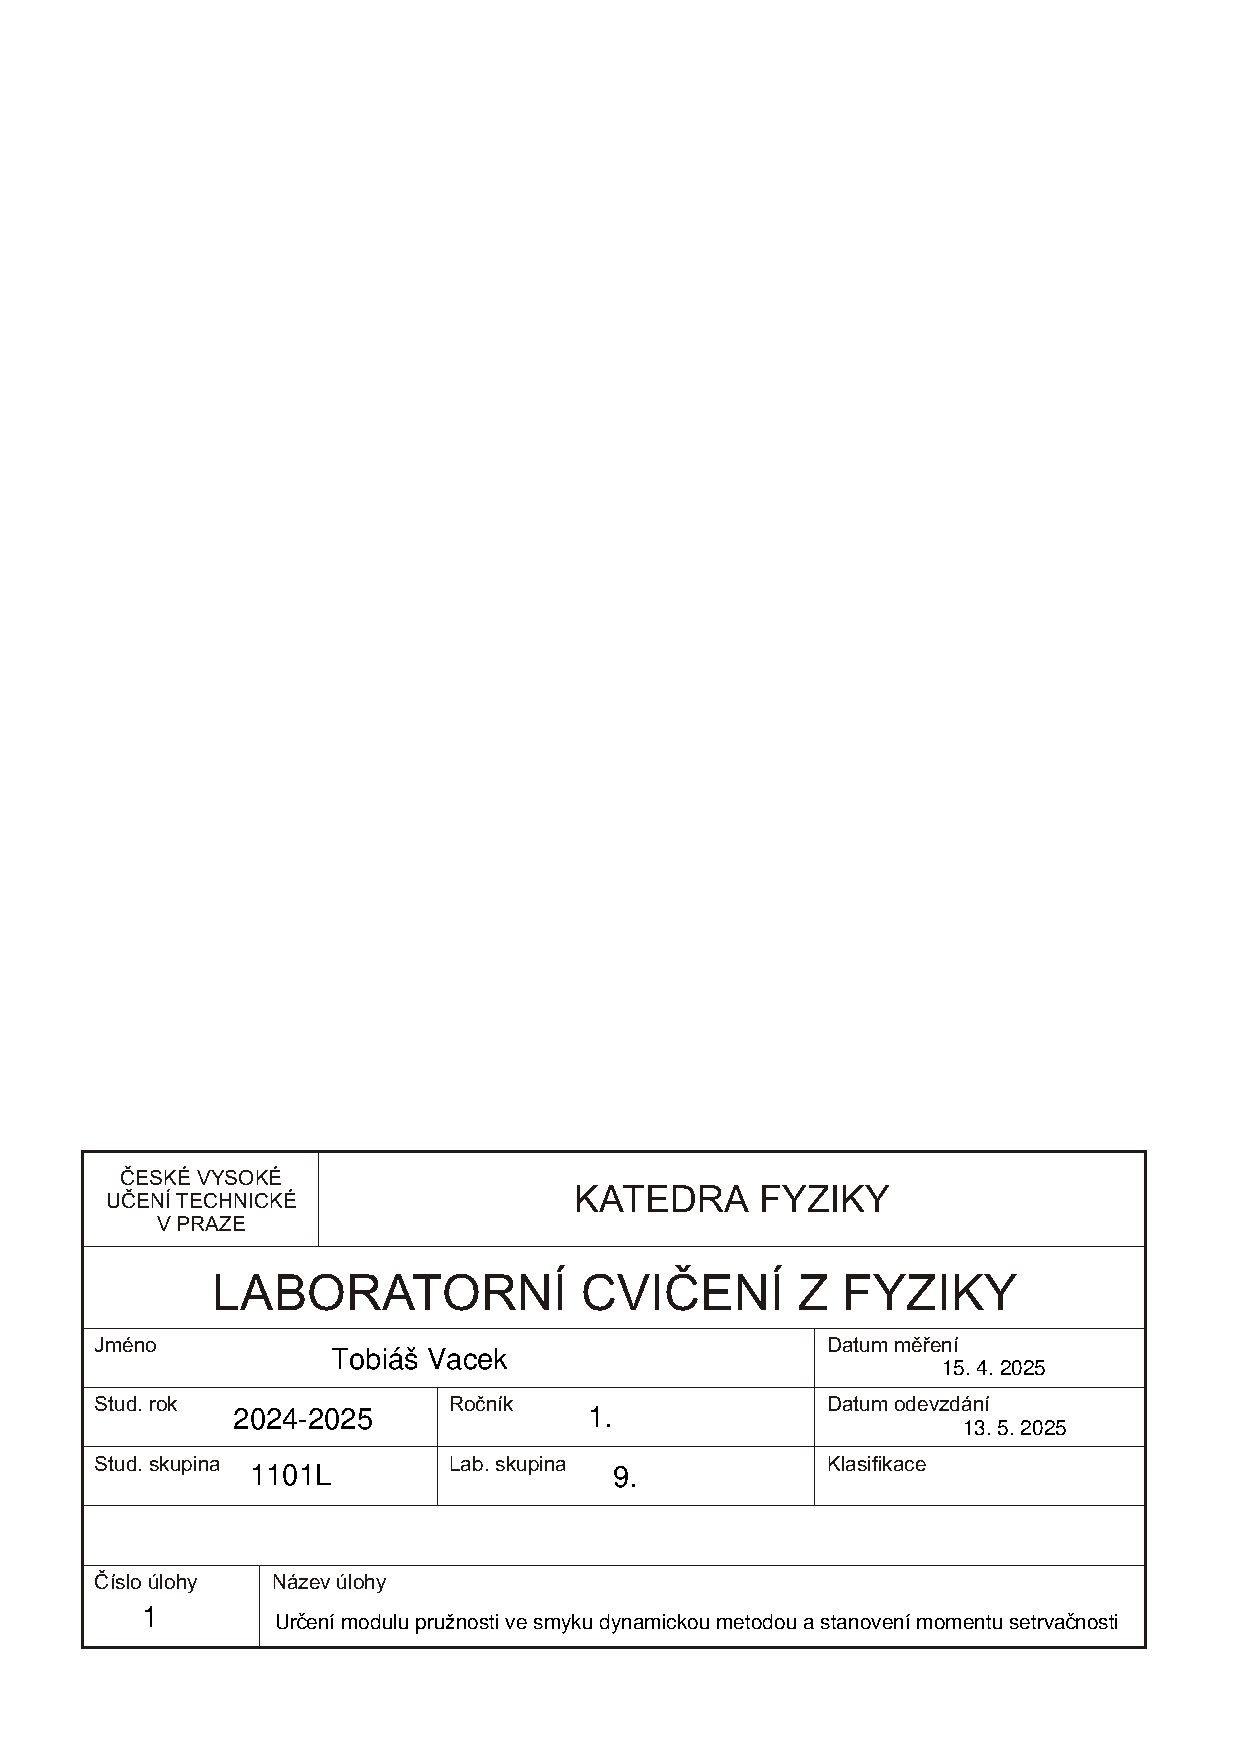
\includepdf{stamp.pdf}

\chapter{Závěr}
\large
Model pružnosti ve smyku ocelové struny jsme pomocí torzního kyvadla spočítali na $G = (8.21\cdot10^{10}\pm0.10\cdot10^{10})\,Pa$, to odpovídá tabulkové hodnotě pro ocel $(7.9-8.9)\cdot10^{10}\,Pa$.
\newline
\newline 

\noindent Po zjistění modelu pružnosti struny, jsme moment setrvačnosti rotoru elektromotoru určili na $(1.88\cdot10^{-3}\pm0.09\cdot10^{-3})\,kg\cdot m^2$ 

\chapter{Literatura}
\begin{enumerate}
  \item https://planck.fel.cvut.cz/praktikum/downloads/navody/torze.pdf
  \item https://planck.fel.cvut.cz/praktikum/downloads/navody/zpracdat.pdf
\end{enumerate}
\end{document}